\chapter{Objective}
\label{chap:Objective}



%%%%%%%%%%%%%%%%%%%%%%%%%%%%%%%%%%%%%%%%%%%%%%%%
%%%%%%%%%  Section: Reconstruction   %%%%%%%%%%%
%%%%%%%%%%%%%%%%%%%%%%%%%%%%%%%%%%%%%%%%%%%%%%%%


\section{Reconstruction}
\label{sec:Reconstruction}

\begin{figure}[h]
    
% RECONSTRUCTION GRAPH
\begin{tikzpicture}[node distance=1cm and 1.7cm, auto]
%%Nodes

\node (D) [minimum height=3.5cm] {\distribution};
\node [above of= D, align=center, yshift=0.7cm] {data set \\ distribution};

\node (A) [node, right= 1cm of D, fill=red!7, yshift=1.5cm] {\textbf{target} \\ $\set A$};
\node (B) [node, right= 1cm of D, yshift=-1.5cm] {\textbf{original} \\ $\set B_\text{true}$};

\node (Bp) [node, right= of B, fill=blue!3] {perturbed \\ \textbf{source} \\ $\set B$}; %\\ $\set B = \delta (\set B_\text{true})$};
\node (Br) [node, right= of Bp, fill=blue!7] {\textbf{reconstructed} \\ $\rho (\set B)$};


%%Arrows
\draw [arrow, dashed, thin] (D) -- (A.190);
\draw [arrow, dashed, thin] (D) -- (B.170);


\draw [arrow, dashed, thin] (B) -- (Bp) 
node (Pert) [midway, function, dashed] {$\delta$};
\draw [linestart] (Bp) -- (Br) 
node (Rec) [midway, function, draw=blue, fill=white] {$\rho$};
\node [fill=white, below= 0cm of Rec] {\color{blue} \footnotesize optimize};
\node [fill=white, below= 0cm of Pert] {\footnotesize \textit{unknown}};


% \draw [dashed] (Rec) to [out=245, in=115] (Rec2);

\node (Net) [function, thick, minimum width= 1cm, above right= -0cm and 3.1cm of A] {$\varphi$};
\node [above right=-0.2cm and 0cm of Net] {\small feature-map};
\node (Loss) [function, thick, above= 1.5cm of Net] {Loss};

\pgfmathtruncatemacro{\OutL}{110}
\pgfmathtruncatemacro{\OutM}{95}
\pgfmathtruncatemacro{\OutR}{75}
\pgfmathtruncatemacro{\InL}{360-\OutL}
\pgfmathtruncatemacro{\InM}{360-\OutM}
\pgfmathtruncatemacro{\InR}{360-\OutR}

\draw [lineend] (Net.\InL) to [corner connect h=-0.7cm] (A.east);
\draw [arrowend] (Net.\OutL) to [out=90, in=270] (Loss.260);

\draw [line] (Net.\InM) to [rect connect h=-0.7cm] (Br.100);
\draw [arrowend] (Net.\OutM) to [out=90, in=270] (Loss.260);

\draw [line, blue] (Net.\InR) to [rect connect h=-0.4cm] (Br.80);
\draw [lineend, blue, connect v] (Net.\OutR) to (Loss.south);
\draw [arrowend, blue, connect h] (Br.192) to (Rec.east);

\path (Net.\OutL) -- node[midway, above= 0.15cm, sloped] {\small statistics}(Loss.260);
% \node [above= 0.5cm of Net, fill=white] {\footnotesize optimize};
% \draw [arrow, Mahogany, thin, bend left=20] (A) to node[near end, above] {\footnotesize trained} (Net);

\node [above= 1cm of B, yshift=-1.5cm] {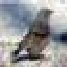
\includegraphics[]{figures/CIFAR10_example.pdf}};

\end{tikzpicture}




% % RECONSTRUCTION GRAPH
% \begin{tikzpicture}[node distance=1cm and 1.7cm, auto]
% %%Nodes

% \node (D) [minimum height=3.5cm] {\distribution};
% \node [above of= D, align=center, yshift=0.7cm] {data set \\ distribution};

% \node (A) [node, right= 1cm of D, fill=red!7, yshift=1.5cm] {\textbf{target} \\ $\set A$};
% \node (B) [node, right= 1cm of D, yshift=-1.5cm] {\textbf{original} \\ $\set B_\text{true}$}

% \node (Bp) [node, right= of B, fill=blue!3] {perturbed \\ \textbf{source} \\ $\set B$}; %\\ $\set B = \delta (\set B_\text{true})$};
% \node (Br) [node, right= of Bp, fill=blue!7] {\textbf{reconstructed} \\ $\rho (\set B)$};


% %%Arrows
% \draw [arrow, dashed, thin] (D) -- (A.190);
% \draw [arrow, dashed, thin] (D) -- (B.170);


% \draw [arrow, dashed, thin] (B) -- (Bp) 
% node (Pert) [midway, function, dashed] {$\delta$};
% \draw [linestart] (Bp) -- (Br) 
% node (Rec) [midway, function, draw=blue, fill=white] {$\rho$};
% \node [fill=white, below= 0cm of Rec] {\color{blue} \footnotesize optimize};
% \node [fill=white, below= 0cm of Pert] {\footnotesize \textit{unknown}};


% % \draw [dashed] (Rec) to [out=245, in=115] (Rec2);

% \node (Net) [function, thick, minimum width= 1cm, above right= -0cm and 3.1cm of A] {$\varphi$};
% \node [above right=-0.2cm and 0cm of Net] {\small feature-map};
% \node (Loss) [function, thick, above= 1.5cm of Net] {loss};

% \pgfmathtruncatemacro{\OutL}{110}
% \pgfmathtruncatemacro{\OutM}{95}
% \pgfmathtruncatemacro{\OutR}{75}
% \pgfmathtruncatemacro{\InL}{360-\OutL}
% \pgfmathtruncatemacro{\InM}{360-\OutM}
% \pgfmathtruncatemacro{\InR}{360-\OutR}

% \draw [lineend] (Net.\InL) to [corner connect h=-0.7cm] (A.east);
% \draw [arrowend] (Net.\OutL) to [out=90, in=270] (Loss.260);

% \draw [line] (Net.\InM) to [rect connect h=-0.7cm] (Br.100);
% \draw [arrowend] (Net.\OutM) to [out=90, in=270] (Loss.260);

% \draw [line, blue] (Net.\InR) to [rect connect h=-0.4cm] (Br.80);
% \draw [lineend, blue, connect v] (Net.\OutR) to (Loss.south);
% \draw [arrowend, blue, connect h] (Br.192) to (Rec.east);

% \path (Net.\OutL) -- node[midway, above= 0.15cm, sloped] {\small statistics}(Loss.260);
% % \node [above= 0.5cm of Net, fill=white] {\footnotesize optimize};
% % \draw [arrow, Mahogany, thin, bend left=20] (A) to node[near end, above] {\footnotesize trained} (Net);


% \end{tikzpicture}


    \caption{Overview}
    \centering
\end{figure}

This section describes the main objective of the task.
The goal is to learn an inverse transformation to the unknown $\delta$.
The way this is achieved is by maximizing similarity between the distributions of a source data set $\set B$
and a target data set $\set A$ in an appropriate feature-space $\phi$.
The goal of maximizing similarity in feature-space is addressed by formulating a loss function
that minimizes simple statistics, such as the mean and variance of the dataset.

Example application:
A neural network might be well adjusted to a target distribution, 
though under-perform when presented with samples that don't follow the original distribution
and exhibit different statistics to which the neural network was not adjusted to.
To combat this problem, a method for readjusting the inputs is introduced.
The basic idea is that the data is mapped to a feature-representation.
In this feature-space, simple statistics, such as the mean and variance are recorded
for both, a source data set $\set B$ and a target data set $\set A$.
Although, the source is first sent through a re-adjustment function $\rho$ that is
then tuned to minimize the similarity-loss of the two data sets.
This is done via a differentiable loss, or objective function that minimizes the difference in statistics.



\subsection{Problem Formulation}
Given: feature-map $\varphi$, target data set $\set A$ (or $\varphi(\set A)$ statistics), and a perturbed data set $\widetilde {\set B}$

\[
    \min_{\rho \in \mathcal{F}} \loss _\varphi (\set A, \rho(\widetilde{\set B})) \,,
\]
where $\mathcal F$ is a pre-defined set of functions.






%%%%%%%%%%%%%%%%%%%%%%%%%%%%%%%%%%%%%%%%%%%%%%%%
%%%%%%%%%%   Section: Inversion    %%%%%%%%%%%%%
%%%%%%%%%%%%%%%%%%%%%%%%%%%%%%%%%%%%%%%%%%%%%%%%


\section{Inversion}
\label{sec:Inversion}

\begin{tikzpicture}[node distance=1.3cm and 1.4cm, auto]

%%Nodes
\node (D) [minimum height=3.5cm] {\distribution};
\node [above of= D, align=center, yshift=0.2cm] {data set \\ distribution};

\node (N) [below= -0.5cm of D, minimum height=3.5cm] {\noise};
\node [above of= N] {random noise};

\node (B) [node, right= of N, fill=blue!7, draw=blue, thick] {\textbf{Source} \\ $\set B$};
\node (A) [node, right= of D, fill=red!7] {\textbf{target} \\ $\set A$};

\path (A) -- (B) node (Mid) [midway] {};
\node (Net) [function, thick, minimum width=1cm, right= of Mid, xshift=1.2cm] {$\varphi$};
\node [below right= 0.1cm and -1.2cm of Net] {\small feature-map};
\node (Loss) [function, thick, right= of Net] {loss};

%%Arrows
% \pgfmathtruncatemacro{\InL}{160}
% \pgfmathtruncatemacro{\InM}{175}
% \pgfmathtruncatemacro{\InR}{195}
% \pgfmathtruncatemacro{\OutL}{360-\InL}
% \pgfmathtruncatemacro{\OutM}{360-\InM}
% \pgfmathtruncatemacro{\OutR}{360-\InR}
\pgfmathtruncatemacro{\OutL}{20}
\pgfmathtruncatemacro{\OutM}{5}
\pgfmathtruncatemacro{\OutR}{-15}
\pgfmathtruncatemacro{\InL}{180-\OutL}
\pgfmathtruncatemacro{\InM}{180-\OutM}
\pgfmathtruncatemacro{\InR}{180-\OutR}

\draw [arrow, dashed, thin] (D) -- (A);
\draw [arrow, dashed, thin] (N) -- (B);

\draw [linestart] (A.east) to [rect connect v=1cm] (Net.\InL);
\draw [arrowend] (Net.\OutL) to[out=0, in=180]  (Loss.170);

\draw [linestart] (B.15) to [rect connect v=1cm] (Net.\InM);
\draw [arrowend] (Net.\OutM) to[out=0, in=180] (Loss.170);

\draw [arrowend, blue] (Net.\InR) to[out=180, in=0, rect connect v=-0.5cm] (B.-5);
\draw [lineend, blue, connect h] (Net.\OutR) to (Loss.west);
\node [below= 0cm of B, yshift=-0cm] {\color{blue} \footnotesize optimize};

\path (Net) -- (Loss) node [above=0.3cm, midway] {\small statistics};
% \draw [arrow, Mahogany, thin, bend left=30] (A.20) to [out=40, in=140] node[above, sloped] {\footnotesize trained} (Net);

\node [below= 0cm of A] {\fbox{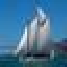
\includegraphics[]{figures/CIFAR10_example_3.pdf}}};

\end{tikzpicture}



The second part of this work is concerned about what kind of data may be recovered from 
having knowledge of the statistics of a data set.
For this task, the goal is to modify the source data set $\set B$ to more closely resemble
the target data set $\set A$ only given the statistics of data set $\set A$.
The source data set $\set B$ is in a first step, initialized by random noise.
Then, by performing gradient descent on the loss function, the source itself is optimized.

Furthermore, the original objective that was used in training the neural network - the \textbf{criterion} - can be used in order to further "push" the samples in a desired direction by specifying individual target labels.



\subsection{Objective}
Given: $\varphi$, $\set A$ (or $\varphi(\set A)$ statistics)
\[
    \min_{\set B \in \powerset Z} \loss _\varphi (\set A, \set B)
\]
    

\subsection{Reconstruction Network}

\begin{minipage}{0.5\textwidth}
\input{Figures/ChartInvertblock}
\end{minipage}
\begin{minipage}{0.5\textwidth}
\begin{tikzpicture}[node distance=0.58cm and 1.7cm, auto]

\node [] (input) {Input};
\node [layer, below= 1cm of input, fill=Dandelion!9] (conv1) {Conv1x1};
\node [layer, below= of conv1] (res1) {Residual Layer};
\node [layer, below= of res1] (res2) {Residual Layer};
\node [below= of res2, minimum height=0.8cm] (res3) {\dots};
\node [layer, below= of res3] (res4) {Residual Layer};
% \node [layer, below= 1cm of input, fill=Dandelion!9] (conv1) {Conv3x3};
% \node [layer, below= of conv1, fill=Blue!5] (bn1) {BatchNorm};
% \node [layer, below= of bn1, fill=Mahogany!7] (relu) {ReLU};
% \node [layer, below= of relu, fill=Dandelion!9] (conv2) {Conv3x3};
% \node [layer, below= of conv2, fill=Blue!5] (bn2) {BatchNorm};
\node [below= 1cm of res4] (output) {Output};

% \path (input) -- node[anchor=center] (branch) {} (conv1);
% \path (bn2) -- node[circle, draw, minimum size=0.6cm, anchor=center] (plus) {} (output);
% \node at (plus) {+};

% \node [right= 1.6cm of branch] (dummy) {};
\node [draw, dashed, inner sep=0.25cm, fit=(res1)] {};

% \draw [larrow, rect connect v=2cm] (branch.center) to (plus.east);

\draw [larrow] (input) to (conv1);
\draw [larrow] (conv1) to (res1);
\draw [larrow] (res1) to (res2);
\draw [larrow] (res2) to (res3);
\draw [larrow] (res3) to (res4);
\draw [larrow] (res4) to (output);
% \draw [larrow] (bn1) to (relu);
% \draw [larrow] (relu) to (conv2);
% \draw [larrow] (conv2) to (bn2);
% \draw [larrow] (bn2) to (plus);
% \draw [larrow] (plus) to (output);


\end{tikzpicture}
\end{minipage}





\subsection{Inversion Evaluation}
The result of the optimization process can be evaluated by calculating the accuracy obtained by $\Phi$. 
Though, since $\Phi$ was used in the optimization process, it will likely display heavy bias to what it believes is a correctly classified sample.
For this sake, another neural network $\Phi_{\text{ver}}$ can be employed, which has been separately trained on either $\set A$ or another data set. Though, practice has shown that a very small portion of $\set A$ is only needed to obtain a close-enough guess at the true statistics of $\set A$.

